Compression can be split into two kinds - lossy and lossless. Using "lossless" in the context of audio is a bit misleading, since sampling itself is a lossy process, but using a high enough sampling rate, we will not notice any difference, so sampled audio without any lossy compression will be our baseline.

For audio, lossless compression generally means taking some form of digital audio representation and losslessly compressing this data. This will preserve the signal in its entirety with a reduced bit-rate. However, due to size of such audio (an audio CD could only fit about 80 minutes of such music sampled at 44.1 kHz), it's become more common to use a lossy format.

Lossy compression implies that there will be loss of data, and while this is true, thanks to the application of various psychoacoustic principles size of audio can be greatly reduced without altering human perception, leading to vastly smaller bit-rates for no real cost.

This work focuses on lossy audio compression, therefore only lossy codecs will be considered for comparison.

\section{Overview}

\section{State of the art}
Due to its qualities of efficiently compacting energy and mitigating artifacts at block boundaries, MDCT is the most commonly used transformation in modern lossy audio coding, and is employed in the most popular audio formats including MP3, Opus, Vorbis or AAC.

In this section, I will elaborate on some of the more popular ones to get an idea of what considerations go into writing a modern audio codec. They are also the ones that will be used for comparison with my own encoding scheme.

\subsection{MP3}
\begin{figure}[ht]
	\caption[MP3 encoding scheme]{The MP3 encoding scheme, simplified.}
	\label{fig:mp3_scheme}
	\centering
	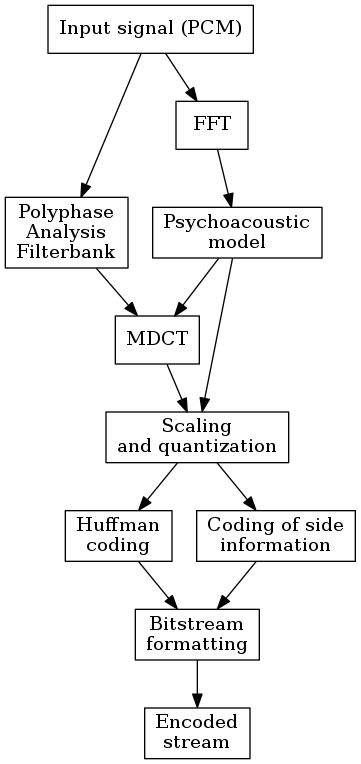
\includegraphics[width=0.45\textwidth]{mp3_scheme.png}
\end{figure}

MP3, or MPEG-1 Layer III has been standardized in 1991 and has since become widespread throughout a multitude of electronic devices as the de-facto standard for music storage. Its simplified encoding scheme can be seen in Figure \ref{fig:mp3_scheme}.

It's a very powerful compression/decompression scheme capable of reducing the bit-rate of an audio stream by up to a factor of 12 without any noticeable (to humans) quality degradation. In other words, to transmit CD quality audio, it needs a bitrate of 128 kbps. \cite{Raissi2002TheTB}

The core of MP3 compression is the Modified discrete cosine transform. The signal represented in its PCM form is first split into 32 subbands using an analysis polyphase filterbank, and each of those is further split into 18 MDCT bins, so overall we end up with 576 MDCT frequency bins per frame.

These bins are then sorted into 22 scalefactor bands, which roughly correlate to the 24 bands of human hearing. The point of these bands is that you may individually scale each of them up or down depending on how much precision you need for that specific frequency range. This usually done by dividing and rounding the values in the band, losing a certain amount of information; this process will be reversed during decoding.

The signal is also analyzed using the Fourier transformation, which gives us frequency information for the signal in the same frame, and we can use this information to determine how much to scale each scalefactor band - e.g. if there's some weak sound that will be masked by another, we can assign the band it's in lower precision, saving data. \cite{wilburn_2007}

Once we have the scaled and quantized data, we use the Huffman encoding to losslessly compress these values, and format this output into the final bitstream, encoding our audio.

\subsection{Opus (CELT)}
The Opus codec has been standardized fairly recently, in 2012 \cite{rfc6716} compared to other widespread audio codecs. Opus was created from two core technologies - Skype's SILK codec based on linear prediction, and Xiph.Org's CELT codec, based on the MDCT. \cite{opus_celt}

As a result, Opus is capable of performing in three different modes:

\begin{description}
	\item[SILK] used for speech signals
	\item[CELT] used for high-bitrate speech and music
	\item[Hybrid] both SILK and CELT used simultaneously
\end{description}

This thesis will mainly focus on Opus CELT due to it being more general purpose than SILK, which will make it easier to use for comparison with a NMF-based codec. SILK uses a technique known as Linear predictive coding, whose complexity and difficulty of implementation exceeds the scope of this work.

Opus is designed with real-time constraints in mind, that is, for example network music performances which require very low delays. Despite that, however, its compression is comparable to codecs with higher delays intended for streaming or storage. This makes it a good candidate to test against in this work, alongside MP3.

CELT (Constrained Energy Lapped Transform) is based on MDCT similar to MP3, but the main difference is that Opus uses specifically sized bands with ranges similar to the Bark scale in order to preserve the spectral envelope of the signal.

Similar to MP3, Opus CELT works on the basis of quantizing MDCT coefficients, but utilizes various kinds of prediction and focuses more on handling transients, and is much more complex in general. Through various optimizations Opus achieves similar results but at a reduced bitrate.

\begin{figure}[ht]
	\caption[Comparison of various audio codecs]{This figure attempts to summarize the results of a collection of listening tests, comparing various lossy audio codecs. Image attributed to \href{http://opus-codec.org/comparison/}{Jean-Marc Valin} and licensed under \href{https://creativecommons.org/licenses/by/3.0/}{CC BY 3.0}.}
	\centering
	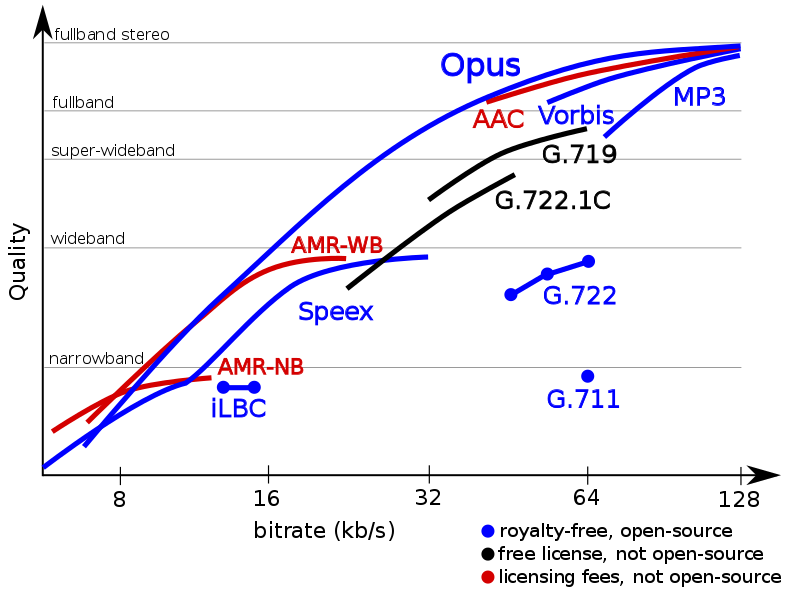
\includegraphics[width=\textwidth]{opus_listening_test.png}
\end{figure}

\section{Compression using NMF}
This section is separate from the state of the art, as NMF is not really used for audio compression in practice. There is one notable example that will be covered and to an extent implemented here, for more details refer to \cite{nikunen_2010}.

The proposed method uses a metric previously formulated in \cite{Nikunen2010NoisetomaskRM} called \emph{noise-to-mask ratio}, or NMR for short. They successfully apply this metric onto non-negative matrix factorization, establishing a custom cost function to represent NMR and also propose update rules based on Euclidean distance for minimizing this cost function.

Results showed that NMR performed better than other, more general cost functions. Audio compressed using NMF + NMR had better perceptual quality and managed to encode signals with lots of transient sounds in better quality. However, NMR relies on proprietary algorithms such as PEAQ \cite{peaq_2006} and an implementation is not readily available.

This modified NMF is then used in what the paper refers to as \emph{object-based audio coding}, and the principle is fairly simple to understand. Instead of using MDCT for conversion to the frequency domain, they use STFT, obtaining the frequency spectrum as a set of complex values. They then take the magnitude and phase of each of these complex values to obtain the \emph{magnitude spectrogram} and \emph{phase information}.

The magnitude spectrogram is then compressed using NMF (+NMR) among other things, whereas the phase information is entropy encoded separately and does not utilize NMF at all.

The conclusion is that while object-based audio coding done this way achieves reasonable bit-rate and quality on the magnitude spectrogram, it is difficult to efficiently encode the phase information and as such the bit-rate of this approach proved to be too high to be usable in practice compared to other, more common, MDCT based methods.

